\documentclass[
    a4paper, % Page size
    fontsize=10pt, % Base font size
    twoside=true, % Use different layouts for even and odd pages (in particular, if twoside=true, the margin column will be always on the outside)
    %open=any, % If twoside=true, uncomment this to force new chapters to start on any page, not only on right (odd) pages
    %chapterentrydots=true, % Uncomment to output dots from the chapter name to the page number in the table of contents
    numbers=noenddot, % Comment to output dots after chapter numbers; the most common values for this option are: enddot, noenddot and auto (see the KOMAScript documentation for an in-depth explanation)
]{kaobook}

\ifxetexorluatex
    \usepackage{polyglossia}
    \setmainlanguage{italian}
\else
    \usepackage[italian]{babel}
\fi
\usepackage[english=british]{csquotes}

% Load packages for testing
\usepackage{blindtext}
%\usepackage{showframe} % Uncomment to show boxes around the text area, margin, header and footer
%\usepackage{showlabels} % Uncomment to output the content of \label commands to the document where they are used

% Load the bibliography package
\usepackage{kaobiblio}
\addbibresource{main.bib} % Bibliography file

% Load mathematical packages for theorems and related environments
\usepackage[framed=true]{kaotheorems}

% Load the package for hyperreferences
\usepackage{kaorefs}

\graphicspath{{examples/documentation/images/}{images/}} % Paths in which to look for images

\makeindex[columns=3, title=Alphabetical Index, intoc] % Make LaTeX produce the files required to compile the index

\makeglossaries % Make LaTeX produce the files required to compile the glossary
\input{glossary.tex} % Include the glossary definitions

\makenomenclature % Make LaTeX produce the files required to compile the nomenclature

% Reset sidenote counter at chapters
%\counterwithin*{sidenote}{chapter}

%----------------------------------------------------------------------------------------

\begin{document}

%----------------------------------------------------------------------------------------
%   BOOK INFORMATION
%----------------------------------------------------------------------------------------
\title{Sulla struttura dati Euler Tour Trees}
\author{Vittorio Porri}
\date{29 Maggio 2026}
\maketitle

%----------------------------------------------------------------------------------------
%   TABLE OF CONTENTS & LIST OF FIGURES/TABLES
%----------------------------------------------------------------------------------------

\begingroup % Local scope for the following commands

% Define the style for the TOC, LOF, and LOT
\setlength{\textheight}{230\hscale} % Manually adjust the height of the ToC pages

% Turn on compatibility mode for the etoc package
\etocstandarddisplaystyle 
\etocstandardlines 

\tableofcontents % Lasciamo solo la Table of Contents

\endgroup

%----------------------------------------------------------------------------------------
%   MAIN BODY
%----------------------------------------------------------------------------------------

\mainmatter % Denotes the start of the main document content, resets page numbering and uses arabic numbers
\setchapterstyle{kao} % Choose the default chapter heading style

%\input{chapters/introduction.tex}

\setchapterpreamble[u]{\margintoc}
\chapter{Euler Tour Trees}
\labch{Introduzione}

In questa tesi esploreremo gli Euler Tour Trees 
(ETT), una struttura dati dinamica introdotta da 
Henzinger e King \cite{HenzingerKing1999}, 
progettata per mantenere informazioni su foreste 
soggette a modifiche strutturali.

L'obiettivo è supportare operazioni di: 
\begin{itemize}
    \item \textbf{link(u,v)}: aggiungere un arco $(u,v)$ unendo due alberi.
    \item \textbf{cut(u,v)}: rimuovere l'arco $(u,v)$ dividendo l'albero in due.
    \item \textbf{isConnected(u,v)}: verificare se $u$ e $v$ appartengono allo stesso albero.
\end{itemize}

A differenza di altre strutture che operano direttamente sui nodi,
gli ETT si basano sulla linearizzazione dell'albero 
tramite cicli di Eulero. Questa rappresentazione
permette di ridurre complessi problemi di connettività 
a semplici manipolazioni di sequenze.

\begin{definition}
Un ciclo euleriano è un percorso in un grafo che inizia e finisce nello stesso nodo passando esattamente una volta per ogni arco.
\end{definition}

\begin{kaobox}[frametitle=Note] 
Poiché gli alberi non hanno veri cicli euleriani, consideriamo ogni arco $e=(u,v)$ come una coppia di archi diretti $(u,v)$ e $(v,u)$.
\end{kaobox}

L'idea della stuttura dati è quella di creare il ciclo euleriano visitando l'albero tramite una ricerca in profondità (DFS) tenendo traccia degli archi attraverso i quali si prosegue nella visita

\begin{marginfigure}
    \centering
    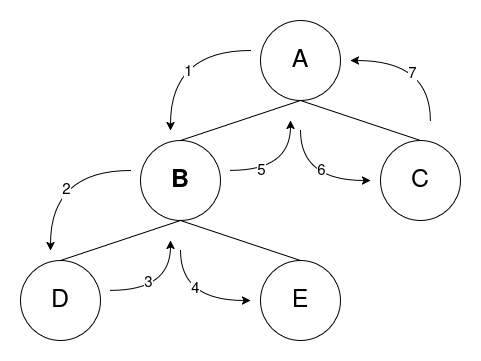
\includegraphics[width=\marginparwidth]{makeTour.png}
    \caption[Ciclo Euleriano]{Il Ciclo euleriano che si forma è (A,B), (B,D), (D,B), (B,E), (E,B), (B,A), (A,C), (C,A)}
    \label{fig:Tour}
\end{marginfigure}

\begin{algorithm}[H]
    \caption{Creazione Tour Euleriano }
    \label{alg:make_ETT}
    \SetAlgoLined
    \DontPrintSemicolon
    
    \KwIn{Nodo corrente $u$, Lista $L$}
    \KwOut{Cammino euleriano in $L$}
    
    \BlankLine 

    \ForEach{figlio $v$ di $u$}{
        $L.append( (u, v) )$ \;
        makeTour($v, L$)\;
        $L.append( (v, u) )$ \;
    }

\end{algorithm}

Il ciclo euleriano è strettamente connesso con la struttra dell'albero, ad esempio si osserva che la sequanza (A,B), \textbf{(B,D), (D,B), (B,E), (E,B)}, (B,A), (A,C), (C,A) rappresenta il sottoalbero radicato in B

\begin{kaobox}[frametitle = Claim]
    Sia $S$ la sequenza di archi che descrive 
    il tour euleriamo per ogni nodo $v$ il 
    sottoalbero radicato in $v$ è rappresenta dall'intervallo 
    contiguo va dal primo arco che ha $(v,\_)$ fino all'ultimo arco che contiene $(\_,v)$    
\end{kaobox}\setchapterpreamble[u]{\margintoc}

\subsection{Operazioni}

\subsubsection{isConnected}
L'operazione \textbf{isConnected(u,v)} è la più semplice poichè è sufficente verificare che i due nodi $u$ e $v$ si trovino nello stesso ciclo euleriano, per farlo basta verificare che il primo elemento della sequanza sia il medesimo per i due nodi.

\subsubsection{Rerooting}
Prima di introdurre le altre operazioni introduciamo,
un'operazione ausiliaria \textbf{rerooting(T,v)}, 
tale operazione ha il compito di rendere un nodo 
interno del ciclo euleriano il primo nodo del ciclo
, per farlo seguiamo i seguenti passaggi:

\begin{enumerate}
    \item si cerca una occorrenza che ha $(v,c)$ (dove $c$ è un figlio casuale di v) nel ciclo euleriano, e si separa la sequanza in A che conterrà tutto ciò che c'era prima di tale arco e B che conterrà l'arco $(v,c)$ e tutto ciò che c'è dopo
    \item riconcateno $B + A + (c,v)$
\end{enumerate}

\begin{algorithm}[H]
    \caption{Rerooting}
    \label{alg:rerooting}
    \SetAlgoLined
    \DontPrintSemicolon
    
    \KwIn{ETT $L$, nodo $v$}
    \KwOut{Il nuovo ETT con radice $v$}
    
    \BlankLine 

    \If{$L[0].source == v$}{
        \Return $L$
    }
    
    $A \leftarrow \emptyset; B \leftarrow \emptyset; isFound \leftarrow False; c \leftarrow NULL$\;
    

    \For{$i \leftarrow 0$ \KwTo $len(L) - 1$}{
        \tcp{Cerchiamo il primo arco che parte da v}
        \If{$L[i].source == v$ \textbf{and} $\neg isFound$}{
            $isFound \leftarrow True$\;
            $c \leftarrow L[i].target$\;
        }

        \If{$\neg isFound$}{
            $A \leftarrow A + L[i]$\;
        }
        \Else{
            $B \leftarrow B + L[i]$\;
        }
    }

    \Return $B + A + (c,v)$
\end{algorithm}

\subsubsection{Link}
L'operazione \textbf{link(u,v)} permette di unire due alberi distinti aggiungendo un arco tra il nodo u (appartenente al primo albero) e il nodo v (appartenente al secondo), per farlo seguiamo i seguenti passaggi:
\begin{enumerate}
    \item A = rerooting(u)
    \item B = rerooting(v) 
    \item concateno  $A + (u,v) + B + (v,u)$ 
\end{enumerate}

\begin{algorithm}[H]
    \caption{Link}
    \label{alg:link}
    \SetAlgoLined
    \DontPrintSemicolon
    
    \KwIn{ETT $L$, ETT $C$, nodo $u$, nodo $v$}
    \KwOut{l'ETT del nuovo albero}
    
    \BlankLine 

    $A \leftarrow rerooting(L,u)$\;
    $B \leftarrow rerooting(C,v)$\;

    \Return $A + (u,v) + B + (v,u)$
    
\end{algorithm}

\subsubsection{Cut}
L'operazione \textbf{cut(u,v)} permette di separare un albero in due alberi distinti, eliminando l'arco $(u,v)$ crando due nuovi alberi radicati rispettivamente in $u$ e $v$, per farlo seguiamo i seguenti passaggi:
\begin{enumerate}
    \item rerooting(T,v)
    \item si cerca la sequanza $(u,v)$ e $(v,u)$ e si separea in A che conterrà tutto ciò che c'era prima di $(u,v)$, B che conterrà $(u,v)$ e $(v,u)$ e tutto ciò che c'è tra i due e C che contiene ciò che c'è dopo $(v,u)$
    \item si eliminano il primo e l'ultimo elemento in $B$
    \item si restituisce $A + C$ e $B$
\end{enumerate}

\begin{algorithm}[H]
    \caption{Cut}
    \label{alg:cut}
    \SetAlgoLined
    \DontPrintSemicolon
    
    \KwIn{ETT $L$, nodo $u$, nodo $v$}
    \KwOut{Due ETT: $L_{rimanente}$ e $L_{staccato}$}
    
    \BlankLine 

    $L \leftarrow \text{rerooting}(L, v)$\;
    
    $A \leftarrow \emptyset; B \leftarrow \emptyset; C \leftarrow \emptyset$\;
    

    \tcp{Trovo il primo arco in cui compare (u,\_)}

    \For{$i \leftarrow 0$ \KwTo $\text{len}(L)-1$}{

        \If{$L[i].source == u$}{
            \textbf{break}\;
        }

        $A \leftarrow A + L[i]$\;

    }

    \tcp{Trova l'ultima arco in cui compare (\_,u)}

    \For{$j \leftarrow \text{len}(L)-1$ \KwTo $0$}{
        \If{$L[j].target == u$}{
            \textbf{break}\;
        }

        $C \leftarrow L[j] + C$\;
    }


    \tcp{Costruisce la sequenza B tra le due occorrenze}

    \For{$k \leftarrow i$ \KwTo $j$}{
        $B \leftarrow B + L[k]$\;
    }

    \text{elimino il primo e l'ultimo elemento di } $B$\;

    \Return $(A + C)$, $B$ 
\end{algorithm}

 \begin{remark}
    Tutte queste implementazioni delle operazioni però hanno costo proporzionale alla dimensione del ciclo euleriano dunque il loro costo sara $O(n)$
 \end{remark}

L'obbiettivo quindi sara quello di introdurre una struttra dati che ci permetterà di eseguire queste operazioni in maniera molto piu efficente


\pagelayout{wide} % No margins
\addpart{Struttura dati}
\pagelayout{margin} % Restore margins
\setchapterpreamble[u]{\margintoc}
\chapter{Balanced Binary Search Trees}
\labch{struttura_dati}

\section{Alberi Binari di Ricerca}
Un Albero Binario di Ricerca (BST) è una struttura dati ad albero che soddisfa le seguenti proprietà per ogni nodo $v$:
\begin{itemize}
    \item Ogni nodo contiene un elemento a cui è associata una chiave presa da un dominio totalmente ordinato.
    \item Tutte le chiavi nel sottoalbero \textbf{sinistro} di $v$ sono minori o uguali ($\leq$) alla chiave in $v$.
    \item Tutte le chiavi nel sottoalbero \textbf{destro} di $v$ sono maggiori o uguali ($\geq$) alla chiave in $v$.
\end{itemize}

\begin{kaobox}[frametitle=Note] 
Eseguendo una visita \textbf{simmetrica} dei nodi, le chiavi vengono enumerate in ordine crescente.
\end{kaobox}

\begin{proof}
La dimostrazione procede per induzione sull'altezza $h$ dell'albero:
\begin{itemize}
    \item \textbf{Caso base} $h=1$: L'albero è composto dalla sola radice e dai due figli foglia. La visita simmetrica visita nell'ordine: figlio sinistro, radice, figlio destro. Date le proprietà del BST, l'ordine è rispettato.
    \item \textbf{Passo induttivo} $h>1$: Supponiamo che la proprietà valga per alberi di altezza inferiore a $h$. Per definizione, la visita simmetrica visita il sottoalbero sinistro $L$, poi la radice $r$ e infine il sottoalbero destro $R$. 
    Per ipotesi induttiva, $L$ e $R$ sono visitati in ordine crescente. Poiché ogni chiave in $L \leq \text{key}(r)$ e ogni chiave in $R \geq \text{key}(r)$, l'intera sequenza risultante sarà ordinata.
\end{itemize}
\end{proof}

\subsection{Operazioni}

\subsubsection{Search}
L'algoritmo di ricerca ricalca il principio della ricerca binaria. Partendo dalla radice, si confronta la chiave cercata $k$ con la chiave del nodo corrente $v$:
\begin{itemize}
    \item Se $k = \text{key}(v)$, la ricerca termina con successo e ritorna.
    \item Se $k < \text{key}(v)$, la ricerca prosegue ricorsivamente nel sottoalbero \textbf{sinistro}.
    \item Se $k > \text{key}(v)$, la ricerca prosegue ricorsivamente nel sottoalbero \textbf{destro}.
\end{itemize}
Se si raggiunge un nodo nullo (\texttt{NULL}), la chiave non è presente nell'albero.

\begin{algorithm}[H]
    \caption{Ricerca in un BST}
    \label{alg:search_bst}
    \SetAlgoLined
    \DontPrintSemicolon
    
    \KwIn{Nodo radice $u$, chiave cercata $k$}
    \KwOut{Il nodo con chiave $k$ o \texttt{NULL}}
    
    \BlankLine 
    
    \While{$u \neq \text{NULL}$}{
        \If{$k == u.key$}{
            \Return $u$\;
        }
        \If{$k < u.key$}{
            $u \leftarrow u.left$\;
        }
        \Else{
            $u \leftarrow u.right$\;
        }
    }
    \Return \texttt{NULL}\;
\end{algorithm}

\subsubsection{Insert}
L'obiettivo dell'inserimento è posizionare un nuovo nodo $u$ come \textbf{foglia}, preservando le proprietà dell'albero. Il procedimento prevede i seguenti passi:
\begin{enumerate}
    \item Si crea il nodo $u$ con i relativi attributi (\textit{elem}, \textit{key}).
    \item Si simula una procedura di \textit{search(key(u))} per individuare il futuro nodo padre.
    \item Una volta individuato il padre, si aggancia $u$ come figlio destro o sinistro in modo da rispettare le proprietà dei BST.
\end{enumerate}

\begin{algorithm}
    \caption{Inserimento in un BST}
    \label{alg:insert_bst}
    \SetAlgoLined
    \DontPrintSemicolon
    
    \KwIn{Nodo radice $r$, nuovo nodo $u$ (già inizializzato)}
    
    \BlankLine 
    
    $y \leftarrow \text{NULL}$ \tcp*{y sarà il padre di u}
    
    \If{$r == \text{NULL}$}{
        $r \leftarrow u$ \tcp*{L'albero era vuoto}
        }
        
    $x \leftarrow r$ 
    
    \While{$x \neq \text{NULL}$}{
        $y \leftarrow x$\;
        \If{$u.key < x.key$}{
            $x \leftarrow x.left$\;
        }
        \Else{
            $x \leftarrow x.right$\;
        }
    }
    
    $u.parent \leftarrow y$\;
    
    \ElseIf{$u.key < y.key$}{
        $y.left \leftarrow u$\;
    }
    \Else{
        $y.right \leftarrow u$\;
    }
\end{algorithm}


\subsubsection{Delete}

L'operazione di cancellazione di un nodo $v$ è la più complessa da implementare quindi prima di definire la cancellazione, è necessario introdurre alcune operazioni ausiliarie fondamentali.

\begin{itemize}
    \item \textbf{Ricerca del minimo (findMin):} Partendo dal nodo radice, si segue ricorsivamente il puntatore \textbf{sinistro}. Il minimo è rappresentato dal primo nodo incontrato il cui puntatore sinistro è \texttt{NULL}.
    \item \textbf{Ricerca del successore (findSuccessor):} Il successore di un nodo $v$ è il nodo con la minima chiave tra tutti i nodi aventi chiave maggiore di $\text{key}(v)$. Si distinguono due casi:
    \begin{enumerate}
        \item \textbf{Se $v$ ha un sottoalbero destro:} il successore è semplicemente il valore minimo di tale sottoalbero (\textit{findMin(v.right)}).
        \item \textbf{Se $v$ non ha un figlio destro:} il successore si trova risalendo l'albero fino a individuare il primo antenato di $v$ tale che $v$ appartenga al suo sottoalbero \textbf{sinistro}.
    \end{enumerate}
\end{itemize}


\begin{algorithm}[H]
    \caption{Ricerca del minimo in un BST}
    \label{alg:findmin_bst}
    \SetAlgoLined
    \DontPrintSemicolon
    
    \KwIn{Nodo radice $r$}
    \KwOut{Il nodo con chiave minima o \texttt{NULL}}
    
    \BlankLine 
    
    \If{$r == \text{NULL}$}{
        \Return \texttt{NULL}\;
    }
    
    $x \leftarrow r$\;
    \While{$x.left \neq \text{NULL}$}{
        $x \leftarrow x.left$\;
    }
    
    \Return $x$\;
\end{algorithm}



\begin{algorithm}[H]
    \caption{Ricerca del successore di un nodo in un BST}
    \label{alg:findSuccessor_bst}
    \SetAlgoLined
    \DontPrintSemicolon
    
    \KwIn{Nodo $v$ di cui cercare il successore}
    \KwOut{Il nodo successore o \texttt{NULL}}
    
    \BlankLine 
    
    \If{$v.right \neq \text{NULL}$}{
        \Return \text{findMin}(v.right)\;
    }
    
    $u \leftarrow v$\;
    \While{$u.parent \neq \text{NULL} \land u.parent.right == u$}{
        $u \leftarrow u.parent$\;
    }
    \Return $u.parent$\;
\end{algorithm}


Le operazioni di cancellazione richiede la gestione di tre scenari differenti:

\begin{itemize}
    \item \textbf{Caso 1: $v$ è una foglia.} Si rimuove il nodo aggiornando il corrispondente puntatore del padre a \texttt{NULL}.
    \item \textbf{Caso 2: $v$ ha un solo figlio.} Si effettua un'operazione di "scavalcamento": il padre di $v$ viene collegato direttamente all'unico figlio di $v$, rimuovendo $v$ dalla struttura.
    \item \textbf{Caso 3: $v$ ha due figli.} Non è possibile rimuovere $v$ direttamente senza rompere la struttura dell'albero. Si procede quindi come segue:
    \begin{enumerate}
        \item Si individua il \textbf{successore} di $v$ (che si troverà necessariamente nel sottoalbero destro).
        \item Si copia il contenuto (chiave ed elementi) del successore nel nodo $v$.
        \item Si rimuove fisicamente il successore dall'albero. Poiché il successore è il minimo del sottoalbero destro, esso avrà al massimo un figlio (il destro), ricadendo quindi nel Caso 1 o nel Caso 2.
    \end{enumerate}
\end{itemize}

\begin{algorithm}[H]
    \caption{Cancellazione di un nodo in un BST}
    \label{alg:delete_bst}
    \SetAlgoLined
    \DontPrintSemicolon
    
    \KwIn{Nodo radice $r$, nodo $v$ da rimuovere}
    
    \BlankLine 
    
    $p \leftarrow v.parent$\;

    \If{$v.left == \text{NULL} \land v.right == \text{NULL}$}{
        \If{$p == \text{NULL}$}{
            $r \leftarrow \text{NULL}$\;
        }
        \ElseIf{$p.left == v$}{
            $p.left \leftarrow \text{NULL}$\;
        }
        \Else{
            $p.right \leftarrow \text{NULL}$\;
        }
    }
    \ElseIf{($v.left == \text{NULL}$) \textbf{xor} ($v.right == \text{NULL}$)}{
        \If{$v.left \neq \text{NULL}$}{
            $child \leftarrow v.left$\;
        }
        \Else{
            $child \leftarrow v.right$\;
        }
        \If{$p == \text{NULL}$}{
            $r \leftarrow child$\;
        }
        \ElseIf{$p.left == v$}{
            $p.left \leftarrow child$\;
        }
        \Else{
            $p.right \leftarrow child$\;
        }
        \If{$child \neq \text{NULL}$}{
            $child.parent \leftarrow p$\;
        }
    }
    \Else{
        $s \leftarrow \text{findSuccessor}(v)$\;
        $v.key \leftarrow s.key$\;
        $v.elem \leftarrow s.elem$\;
        \text{Delete}(r, s)\;
    }
\end{algorithm}

\begin{kaobox}[frametitle=Note] 
Tutte le operazioni dipendono dall'altezza dell'albero per cui il loro costo è $O(h)$
\end{kaobox}

\section{Red-Black Trees}
Lo standard per garantire l'efficienza di queste operazioni è imporre una \textit{condizione di bilanciamento}. Tale vincolo assicura che l'altezza dell'albero rimanga logaritmica rispetto al numero di nodi ($h = O(\log n)$), evitando la degenerazione della struttura in una lista concatenata.
Per farlo ad ogni nodo viene associata una funzione chiamata \textbf{rango} che assegna ad ogni nodo $x$ un valore intero non negativo $rank(x)$ che deve soddisfare le seguenti proprietà fondamentali:

\begin{enumerate}
    \item \textbf{Proprietà del Padre:} Se $x$ è un nodo dotato di genitore $p(x)$, allora:
    \[ rank(x) \leq rank(p(x)) \leq rank(x) + 1 \]
    \item \textbf{Proprietà del Nonno:} Se $x$ è un nodo dotato di un nonno $p^2(x)$, allora:
    \[ rank(x) < rank(p^2(x)) \]
    \item \textbf{Proprietà dei Nodi Esterni:} Se $x$ è un nodo esterno (nodo con valore NULL), allora $rank(x) = 0$. Inoltre, se $x$ possiede un genitore, allora $rank(p(x)) = 1$.
\end{enumerate}

Come visto in \cite{tarjan1983data} è possibile derivare una definizione alternativa, ma formalmente equivalente, basata sulla colorazione dei nodi. Si definisce un nodo $x$ come \textbf{Nero} (\textit{Black}) se $rank(p(x)) = rank(x) + 1$ (o se $x$ è la radice dell'albero) e \textbf{Rosso} (\textit{Red}) se $rank(p(x)) = rank(x)$. 


Sotto questa formalizzazione, le condizioni di bilanciamento si traducono nelle proprietà canoniche dei \textbf{Red-Black Trees}:

\begin{enumerate}
    \item Ogni nodo è marcato con il colore rosso o nero.
    \item Un nodo rosso deve necessariamente avere un genitore e un figlio di colore nero.
    \item Ogni nodo esterno è nero e tutti i cammini che congiungono un nodo $x$ ai nodi esterni discendenti contengono il medesimo numero di nodi neri.
    \item La radice dell'albero è nera
\end{enumerate}

\begin{kaobox}[frametitle=Note]
$rank(v) = k$ è il numero di nodi neri che si incontrano dal nodo $v$, escluso, verso qualsiasi sua foglia
\end{kaobox} 

\begin{lemma}
Un albero binario bilanciato con $n$ nodi interni ha altezza  $h \leq 2\log_2(n+1)$.
\end{lemma}

\begin{proof}
Dimostriamo per induzione sul rango $k$ che un nodo $u$ con $rank(u) = k$ possiede un numero di discendenti interni $n(u) \geq 2^k - 1$, poi da qui determiniamo l'altezza dell'albero.

\begin{itemize}
    \item \textbf{Caso base} ($k = 0$): per la Proprietà dei Nodi Esterni, un nodo con rango $0$ è un nodo esterno. Esso non possiede discendenti interni, coerentemente con la formula: $2^0 - 1 = 0$.
    
    \item \textbf{Passo induttivo} ($k > 0$): Supponiamo che la proprietà sia vera per tutti i nodi con rango inferiore a $k$. Sia $u$ un nodo con $rank(u) = k$ e siano $v$ e $w$ i suoi figli. 
    Per la \textit{Proprietà del Padre}, il rango di un figlio può essere $k$ o $k-1$. Tuttavia, analizziamo i due scenari possibili per un generico figlio $v$:
    \begin{enumerate}
        \item Se $rank(v) = k-1$, per ipotesi induttiva $v$ ha almeno $2^{k-1}-1$ discendenti.
        \item Se $rank(v) = k$, allora $v$ deve essere necessariamente un nodo rosso. Per la \textit{Proprietà del Nonno}, i figli di $v$ (nipoti di $u$) devono avere rango strettamente inferiore a $rank(u)$, ovvero $k-1$. In questo caso, applicando l'ipotesi induttiva ai due figli di $v$, il numero di discendenti di $v$ è almeno $(2^{k-1}-1) + (2^{k-1}-1) + 1 = 2^k - 1$.
    \end{enumerate}
    
    In entrambi i casi, ogni figlio di $u$ garantisce almeno $2^{k-1}-1$ discendenti. Sommando i contributi dei due figli di $u$ e del nodo $u$:
        \[ n(u) \geq (2^{k-1} - 1) + (2^{k-1} - 1) + 1 = 2 \cdot 2^{k-1} - 1 = 2^k - 1 \]
\end{itemize}
La proprietà è dunque dimostrata per ogni $k$.\;

Sia $T$ un albero con $n$ nodi interni e sia $k$ il rango della sua radice. Dalla proprietà appena dimostrata sappiamo che:
\[ n \geq 2^k - 1 \]
Risistemando i termini
\[ n + 1 \geq 2^k \implies \log_2(n+1) \geq k \]

Dalla \textit{Proprietà del Nonno}, sappiamo che lungo ogni cammino non possono esserci due nodi rossi consecutivi. Questo implica che l'altezza fisica $h$ dell'albero può essere al massimo il doppio del rango della radice ($h \leq 2k$). 

Sostituendo la relazione trovata per $k$:
\[ h \leq 2k \leq \log_2(n+1) \]
\end{proof}

Le operazioni di inserimento (Insert) e di cancellazione (Delete) sono le medesime degli alberi binari tuttavia potrebbero rovinare il bilanciamento e violare le proprietà dell'albero quindi abbiamo bisogno di alcune operazioni ausiliarie che ripristino tutte le proprietà dei red-blak trees 

\subsubsection{Rotazioni e Ribilanciamento}

Le rotazioni sono operazioni locali che modificano la struttura dell'albero preservando l'ordine simmetrico dei nodi (proprietà di ricerca). Un nodo $v$ intuitivamente è \textbf{sbilanciato} se uno dei suoi sottoalberi è troppo alto rispetto agli alti.

Sia $v$ il nodo sbilanciato possiamo distinguiamo quattro casi fondamentali in base alla posizione del sottoalbero $T$ che causa lo sbilanciamento:

\begin{description}
    \item[Caso Sinistro-Sinistro (SS):] $T$ è il figlio sinistro del figlio sinistro di $v$. Si risolve con una \textit{rotazione semplice verso destra} su $v$.
    \begin{center}
        \nopagebreak 
        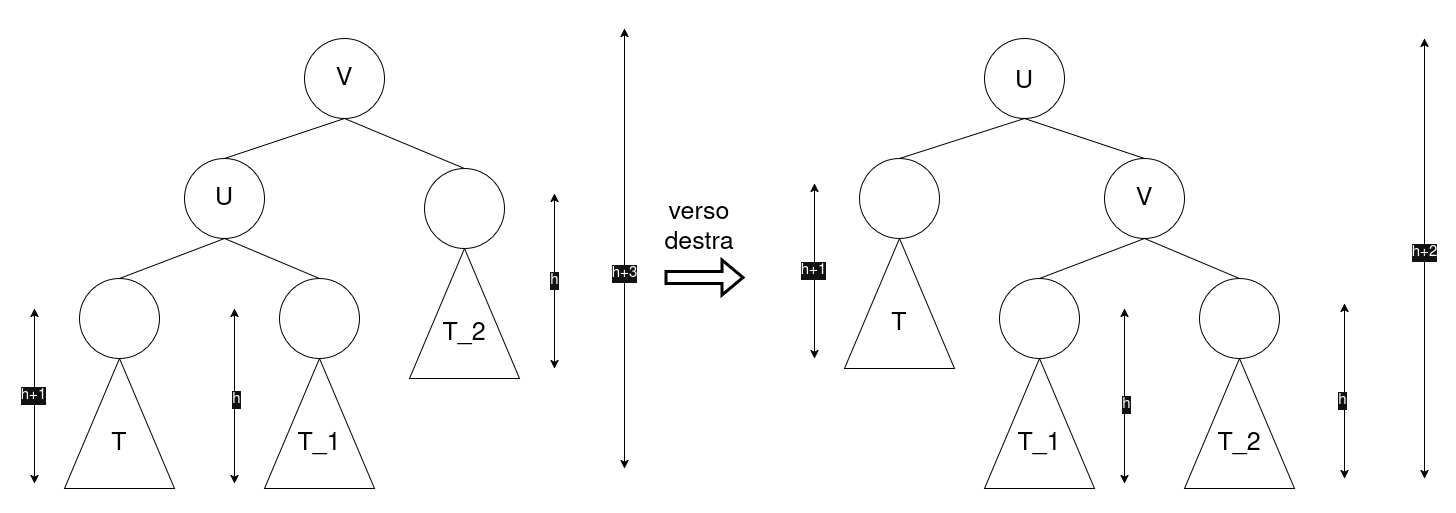
\includegraphics[width=0.8\textwidth]{rotazioneSS.png}
        \captionof{figure}{Rotazione semplice destra (Caso SS).}
        \label{fig:rotazioneSS}
    \end{center}

    \item[Caso Destro-Destro (DD):] Speculare al caso SS. Si risolve con una \textit{rotazione semplice verso sinistra} su $v$.

    \item[Caso Sinistro-Destro (SD):] $T$ è il figlio destro del figlio sinistro di $v$. Si risolve con una \textit{rotazione doppia} (una rotazione verso sinistra sul figlio z, seguita da una verso destra su $v$).
    \begin{center}
        \nopagebreak
        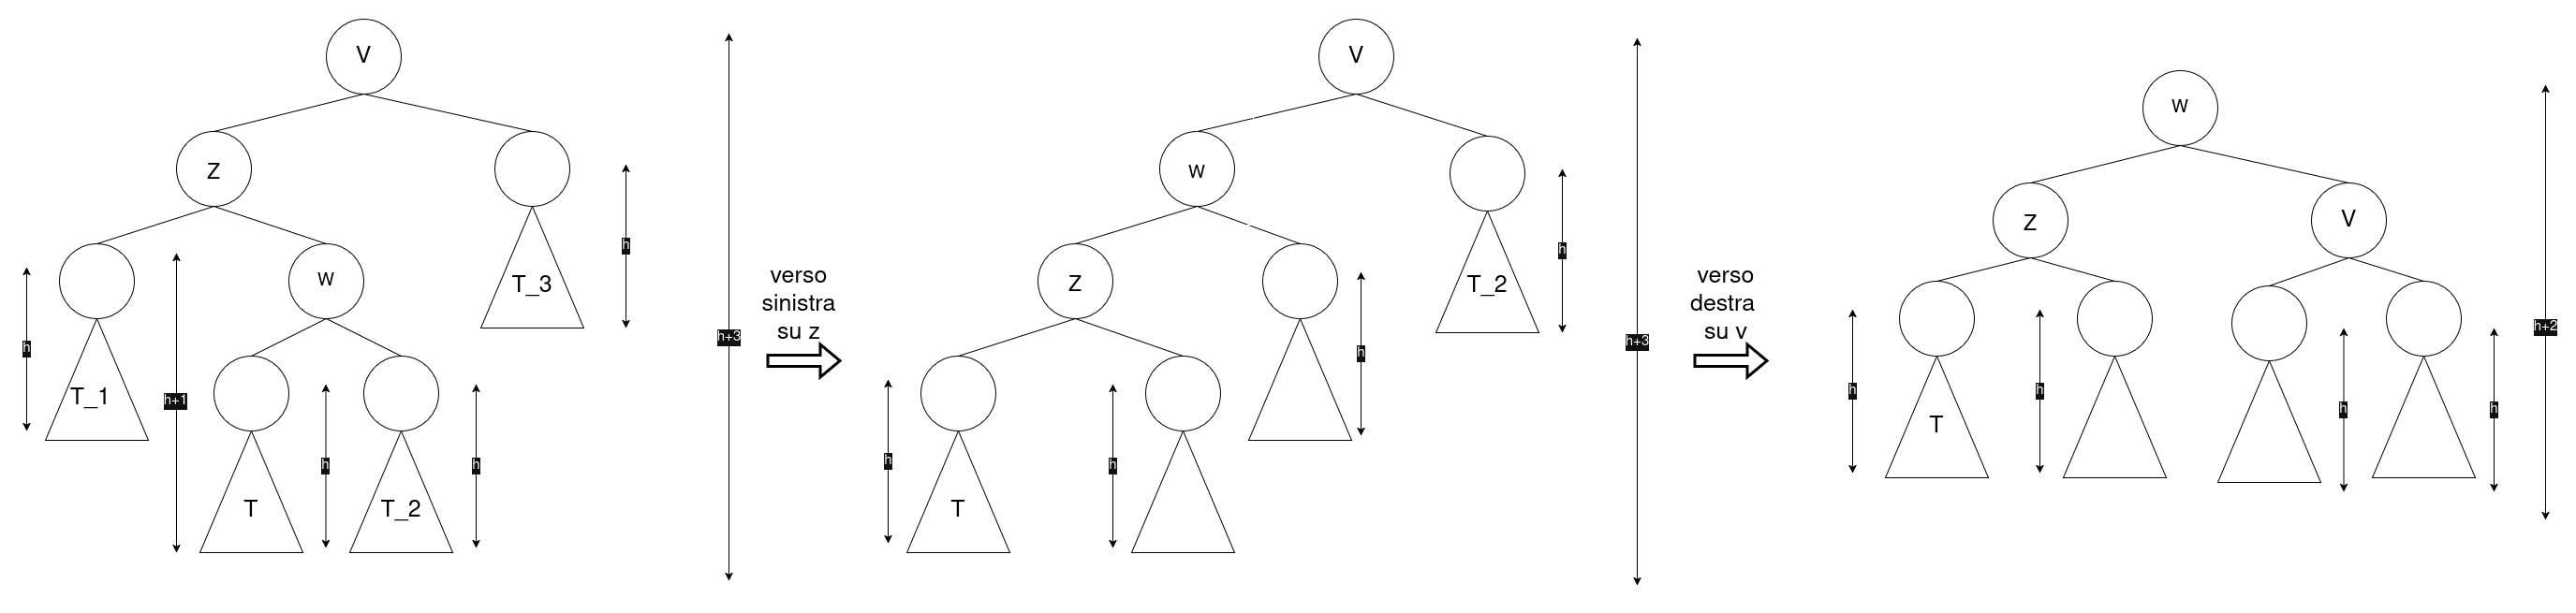
\includegraphics[width=0.9\textwidth]{rotazioneSinistroDestro.png}
        \captionof{figure}{Rotazione doppia sinistra-destra (Caso SD).}
        \label{fig:rotazioneSD}
    \end{center}

    \item[Caso Destro-Sinistro (DS):] Speculare al caso SD. Si risolve con una rotazione doppia destra-sinistra.
\end{description}

\begin{lemma}
    Sia $v$ un nodo sbilanciato a seguito di un'operazione di inserimento o cancellazione. Esiste sempre una rotazione semplice o doppia in grado di ripristinare il bilanciamento del sottoalbero radicato in $v$.
\end{lemma}

\begin{proof}
    Si consideri il caso Sinistro-Sinistro (Fig. \ref{fig:rotazioneSS}). Prima della rotazione, l'altezza del sottoalbero radicato in $v$ è $h+3$. Dopo la rotazione semplice destra, il nodo $u$ diventa la nuova radice locale. La nuova altezza sarà $h+2$\\
    Ragionamento analogo può essere applicato alla rotazione doppia (Fig. \ref{fig:rotazioneSD}), dove la sequenza di rotazioni trasforma un cammino critico di altezza $h+3$ in una struttura bilanciata di altezza $h+2$. \\
    Poiché l'altezza viene ridotta esattamente del valore necessario a compensare lo sbilanciamento e l'ordinamento simmetrico è preservato, il nodo risulta correttamente ribilanciato.
\end{proof}

\subsubsection{Insert}

L'inserimento di un elemento in un \textit{Red-Black Tree} (RBT) è un'operazione composta che integra la logica strutturale degli alberi binari di ricerca con un protocollo di ripristino delle proprietà cromatiche.

Sia $v$ il nodo da inserire nell'albero $T$, si colora il nodo $v$ di \textbf{rosso} e si seguendo l'algoritmo di inserimento standard per i BST.

\paragraph{Analisi della politica di colorazione}
La scelta di assegnare il colore rosso al nuovo nodo $v$ è dettata dalla necessità di limitare le potenziali violazioni alle proprietà strutturali dell'RBT:

\begin{itemize}
    \item \textbf{Invarianza dell'Altezza Nera (Proprietà 3):} L'assegnazione del colore rosso garantisce intrinsecamente il mantenimento della \textit{Proprietà 3}, la quale impone che ogni cammino semplice da un nodo a una foglia discendente contenga il medesimo numero di nodi neri. Poiché $v$ è rosso, il conteggio dei nodi neri (la cosiddetta \textit{black-height}) per ogni cammino che attraversa $v$ rimane inalterato rispetto alla configurazione precedente l'inserimento.
    \item \textbf{Vincoli di Adiacenza (Proprietà 2):} Le unice potenziali violazioni introdotte possono essere releative al fatto che il nodo padre (p(v)) è \textit{NULL} o alla \textit{Proprietà 2}, che vieta la presenza di due nodi rossi consecutivi. Tale conflitto si manifesta esclusivamente nell'eventualità in cui il padre del nodo inserito, $p(v)$, sia a sua volta di colore rosso, in questo caso va utilizzata la procedura fixInsert al fine ripristinare le proprietà dell'albero.
\end{itemize}

\subsubsection{fixInsert}

\begin{marginfigure}
    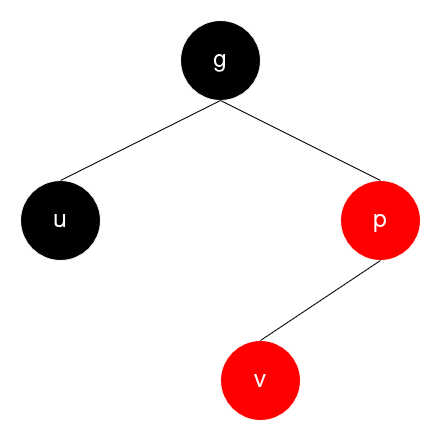
\includegraphics{triangoloDS.png}
    \caption[Titolo breve]{Caso del triangolo destro}
    \labfig{triangolo-destro}
\end{marginfigure}

\begin{marginfigure}
    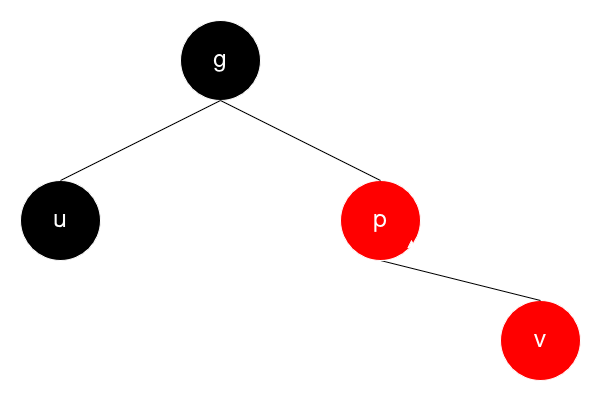
\includegraphics{lineaDestra.png}
    \caption[Titolo breve]{Caso della linea destra}
    \labfig{linea-destra}
\end{marginfigure} 

La routine \texttt{fixInsert(v)} interviene quando il padre del nodo appena inserito, $p[v]$, è rosso o, violando la \textit{Proprietà 2}. Il comportamento della procedura dipende dal colore e dalla posizione dello \textbf{zio} di $v$ , indicato come $u$ (fratello di $p[v]$).

Si distinguono i seguenti casi fondamentali:

\begin{enumerate}
    \item \textbf{Caso della Radice:} Se $p[v]$ è \texttt{NULL}, significa che $v$ è la radice dell'albero. In questo caso è sufficiente ricolorare $v$ di nero per soddisfare tutte le proprietà.
    
    \item \textbf{Ricolorazione (Zio Rosso):} Se lo zio $u$ è rosso, il nonno $g$ deve essere necessariamente nero (\textit{Proprietà 2}). Si procede ricolorando $p[v]$ e $u$ di nero, e $g$ di rosso. 
    \begin{itemize}
        \item \textit{Nota:} Poiché $g$ è diventato rosso, la violazione potrebbe essersi spostata verso l'alto. La procedura viene quindi chiamata ricorsivamente su $g$.
    \end{itemize}

    \item \textbf{Caso del Triangolo :} Se lo zio $u$ è nero (o \texttt{NULL}) e $v$ è un figlio interno rispetto al nonno (es. $v$ è figlio destro e $p[v]$ è figlio sinistro, come in Fig. \ref{fig:triangolo-destro}), ci troviamo in una configurazione a "triangolo". 
    Si applica una \textbf{rotazione semplice} sul padre $p[v]$ per ricondursi al caso della linea (Caso 4).

    \item \textbf{Caso della Linea:} Se lo zio $u$ è nero (o \texttt{NULL}) e $v$ è un figlio esterno (es. entrambi figli sinistri, come in Fig. \ref{fig:linea-destra}), i nodi sono allineati. 
    Si applica una \textbf{rotazione semplice} sul nonno $g$, ricolorando il padre $p[v]$ di nero e il nonno $g$ di rosso. Questa operazione risolve definitivamente la violazione senza alterare la \textit{black-height}.
\end{enumerate}

\begin{remark}
    È importante notare che, mentre il Caso 2 può propagare la violazione fino alla radice con costo $O(\log n)$, i Casi 3 e 4 richiedono al massimo due rotazioni totali per terminare l'esecuzione della procedura.
\end{remark}

\subsubsection{Delete}
L'operazione di rimozione di un nodo in un \textit{Red-Black Tree} segue inizialmente la logica strutturale della cancellazione negli alberi binari di ricerca (BST). Tuttavia, le implicazioni cromatiche variano drasticamente in base al colore del nodo rimosso o del nodo che ne prende il posto:

\begin{itemize}
    \item Se il nodo rimosso è \textbf{rosso}, le proprietà dell'albero rimangono invariate, poiché l'altezza nera dei cammini non subisce alterazioni e non si possono creare conflitti tra nodi rossi consecutivi.
    \item Se il nodo rimosso è \textbf{nero}, si verifica una violazione della \textit{Proprietà 3}, poiché ogni cammino che attraversava quel nodo vedrà ridursi il proprio numero di nodi neri di un'unità.
\end{itemize}

Per ovviare a questa violazione, si introduce una procedura ausiliaria chiamata fixDelete che si occupa di ribilanciare la black-height

\subsubsection{fixDelete}

La procedura \texttt{fixDelete(x)} viene invocata qualora il nodo rimosso sia di colore nero, determinando una violazione della \textit{Proprietà 3} (altezza nera). L'obiettivo della routine è eliminare tale riduzione risalendo l'albero o assorbendola tramite rotazioni.

Il comportamento dell'algoritmo è determinato dal colore del fratello $f$ e dei relativi figli (nipoti di $x$): $cl$ (figlio sinistro) e $cr$ (figlio destro).

\begin{marginfigure}
    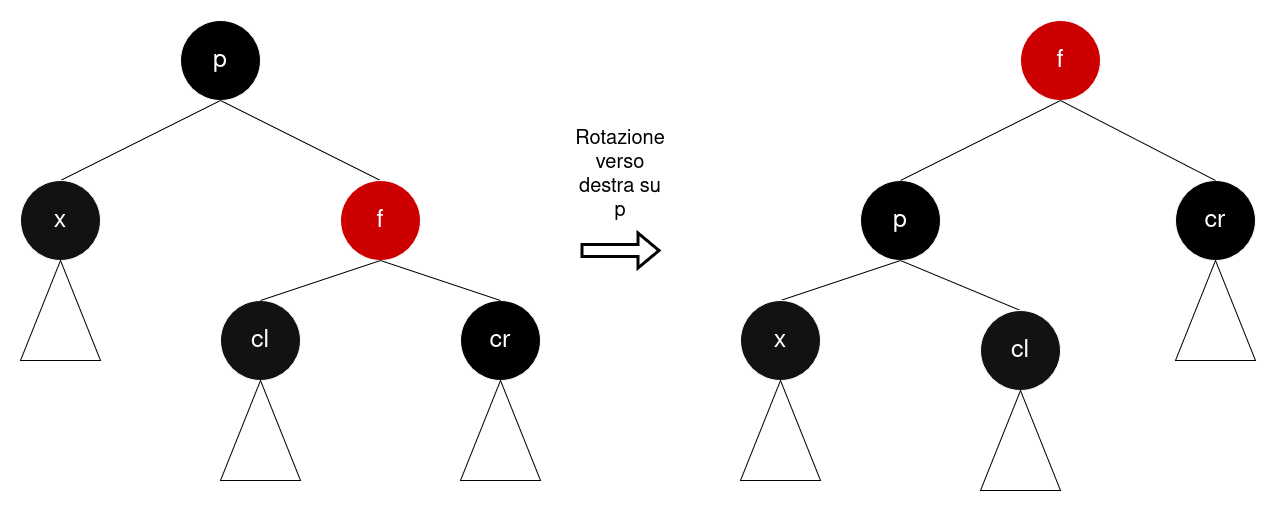
\includegraphics{fratelloRosso.png}
    \caption[Titolo breve]{Caso del fratello Rosso}
    \labfig{fratello-rosso}
\end{marginfigure}

\begin{marginfigure}
    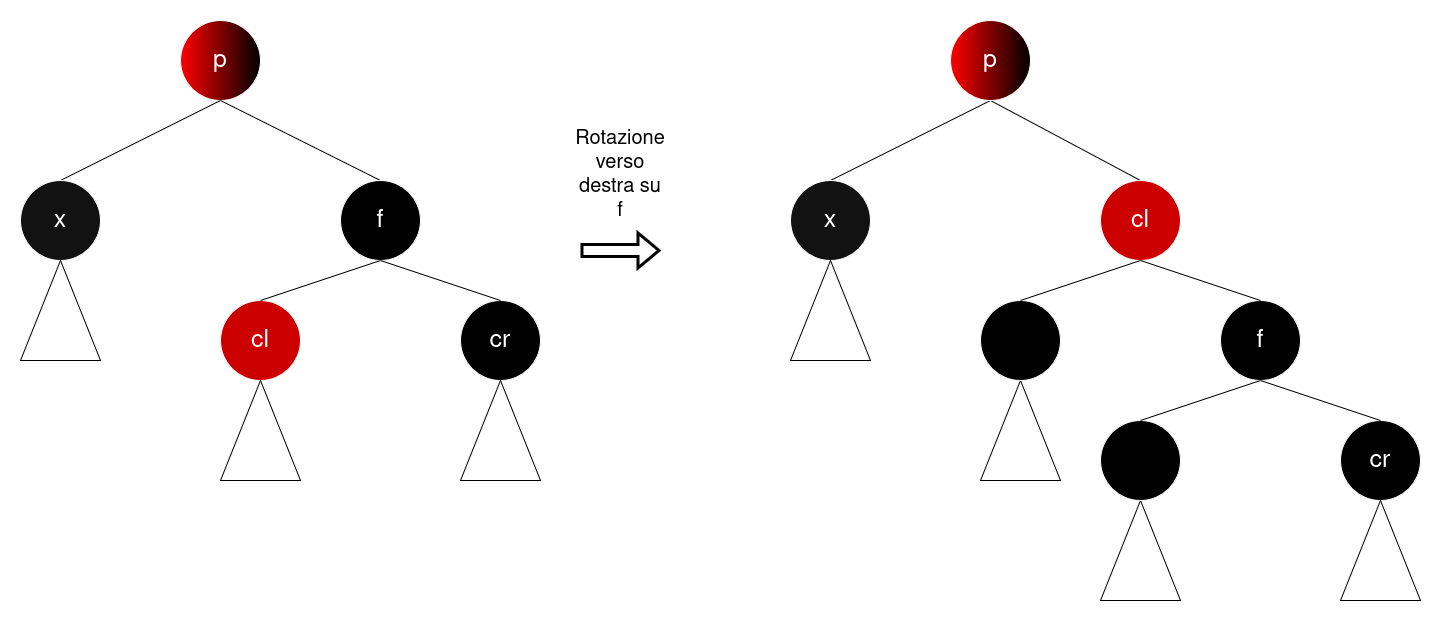
\includegraphics{nipoteVicinoRosso.png}
    \caption[Titolo breve]{Caso del nipote vicino rosso}
    \labfig{nipote-vicino-rosso}
\end{marginfigure}

\begin{marginfigure}
    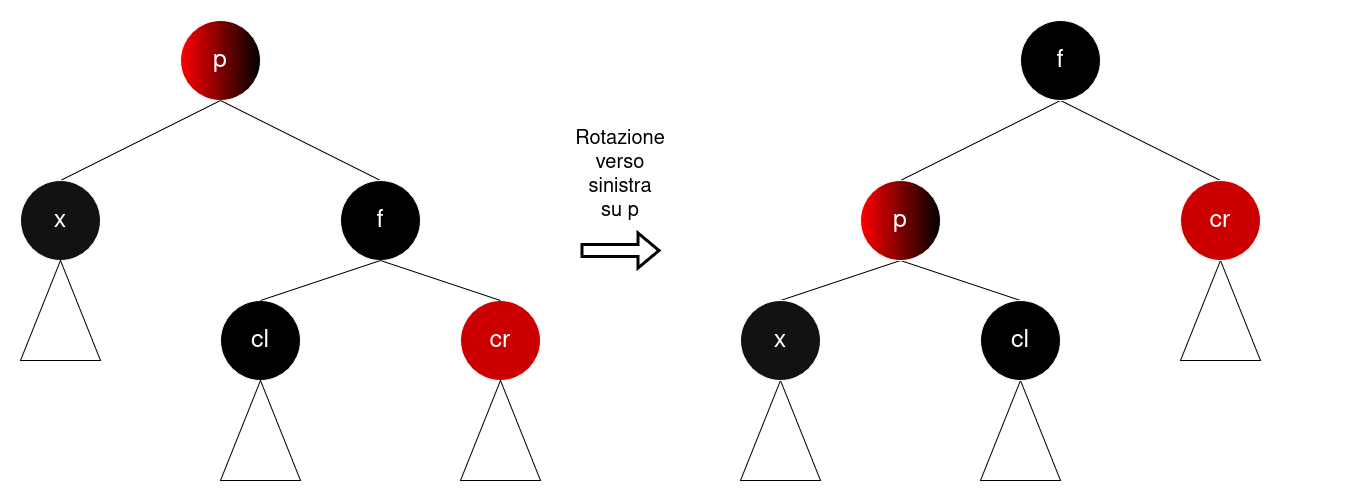
\includegraphics{nipoteLontanoRosso.png}
    \caption[Titolo breve]{Caso del nipote lontano rosso}
    \labfig{nipote-lontano-rosso}
\end{marginfigure}

\begin{enumerate}
    \item \textbf{Caso 1: Fratello $f$ rosso.}
    Se $f$ è rosso, il padre $p[x]$ deve essere necessariamente nero. Si esegue una rotazione (sinistra se $x$ è figlio sinistro, destra se $x$ è figlio destro come nel \ref{fig:fratello-rosso}) su $p[x]$ e si scambiano i colori tra $p[x]$ e $f$. Questa operazione trasforma la configurazione in uno dei casi 2, 3 o 4, dove il nuovo fratello di $x$ è nero.

    \item \textbf{Caso 2: Fratello $f$ e nipoti entrambi neri.}
    In questa situazione, vengono ricolorati $x$ e da $f$ di rosso ora controllo $p[x]$. 
    \begin{itemize}
        \item Se $p[x]$ era rosso, esso diventa semplicemente nero e la procedura termina.
        \item Se $p[x]$ era già nero, allora la procedura \texttt{fixDelete} viene richiamata ricorsivamente verso l'alto su $p[x]$.
    \end{itemize}

    \item \textbf{Caso 3: Nipote "vicino" rosso (Zio nero).}
    Si verifica quando il figlio di $f$ più prossimo a $x$ è rosso (es. $x$ è figlio sinistro e $cl$ è rosso come nella figura \ref{fig:nipote-vicino-rosso}). Si esegue una rotazione su $f$ (direzione opposta a $x$) e si scambiano i colori tra $f$ e il nipote rosso. Questa trasformazione riconduce l'albero al Caso 4.

    \item \textbf{Caso 4: Nipote "lontano" rosso (Zio nero).}
    Si verifica quando il figlio di $f$ più distante da $x$ è rosso (es. $x$ è figlio sinistro e $cr$ è rosso come nella figura \ref{fig:nipote-lontano-rosso}). Si esegue una rotazione su $p[x]$ verso $x$. 
    \begin{itemize}
        \item Il nodo $f$ (nuova radice locale) assume il colore che aveva $p[x]$ prima della rotazione.
        \item I nodi $p[x]$ e il nipote lontano rosso vengono colorati di nero.
    \end{itemize}
    Questa operazione ripristina l'altezza nera.
\end{enumerate}

\begin{kaobox}[frametitle=Note] 
Nei casi 3 e 4, il colore di $p$ può essere sia rosso che nero.
\end{kaobox}

\begin{remark}
    Si osservi che, mentre il Caso 2 può propagare la violazione fino alla radice con costo $O(\log n)$, i Casi 3 e 4 garantiscono la terminazione della procedura dopo un numero costante di rotazioni.
\end{remark}


\subsubsection{Join}

L'operazione di \textbf{Join} riceve in input due alberi Red-Black $S_1$ e $S_2$ e un nodo con chiave $i$, sotto l'ipotesi che:
\[ \forall x \in S_1, \forall y \in S_2 : \text{key}(x) < i < \text{key}(y) \]


L'algoritmo si divide in due casi:
\begin{itemize}
    \item \textbf{Caso $rank(S_1) \geq rank(S_2)$}: 
    Poiché $i$ e tutti gli elementi di $S_2$ sono maggiori di ogni chiave in $S_1$, l'obiettivo è inserire il blocco $(i, S_2)$ all'interno di $S_1$.
    \begin{enumerate}
        \item \textbf{Ricerca}: Si discende lungo il cammino dei figli destri di $S_1$ fino a individuare un nodo $x$ tale che $rank(x) = rank(S_2)$.
        \item \textbf{Innesto}: Sia $p$ il padre di $x$. Il nodo $i$ viene inserito come nuovo figlio destro di $p$, $x$ diventa il figlio sinistro di $i$, mentre la radice di $S_2$ diventa il figlio destro di $i$.
        \item \textbf{Colorazione}: Il nodo $i$ viene colorato di \textbf{rosso}. Affinché la proprietà del rango sia preservata, le radici dei due sottoalberi $x$ e $S_2$ vengono ricolorate di nere.
        \item \textbf{Ribilanciamento}: Viene invocata la procedura \texttt{fixInsert(i)} per risolvere eventuali violazioni della \textit{Proprietà 2}
    \end{enumerate}

    \item \textbf{Caso $rank(S_1) < rank(S_2)$}:
    Il procedimento è simmetrico, ma questa volta si discende lungo il cammino dei figli sinistri di $S_2$ fino a trovare un nodo $x$ con $rank(x) = rank(S_1)$. Il nodo $i$ ( colorato di rosso) sostituirà $x$, prendendo $S_1$ come figlio sinistro e $x$ come figlio destro, poi si ricolora $x$ e $S_1$ di \textbf{nero} e si richiama fixInsert(i)
\end{itemize}
\begin{definition}
    Il costo del  $join(S_1, i, S_2)$ è $O(log(n))$
\end{definition}
\begin{proof}
    La complessità temporale della procedura di $join(S_1, i, S_2)$ dipende dalla ricerca del nodo $x$, che richiede $|rank(S_1) - rank(S_2)|$, $O(1)$ per agganciare l'albero e la procedura \texttt{fixInsert}, richiede tempo proporzionale a quanto siamo discesi nell'albero $|rank(S_1) -rank(S_2)|$ \\
    Quindi, il costo complessivo è $O(|rank(S_1) - rank(S_2)| +1) = O(log(n))$.
\end{proof}

\begin{kaobox}[frametitle=Note] 
    Il rank del nuovo albero che si formerà dopo $\text{join}(S_1, i, S_2)$ sarà:
    \begin{itemize}
        \item Se $\text{rank}(S_1) = \text{rank}(S_2)$, allora il nuovo rank sarà $\text{rank}(S_1) + 1$.
        \item Se $\text{rank}(S_1) \neq \text{rank}(S_2)$, allora il nuovo rank sarà $\max(\text{rank}(S_1), \\\text{rank}(S_2))$.
    \end{itemize}
\end{kaobox}
\newpage
\subsubsection{Split}
L'operazione di \texttt{split}$(T, v)$ divide l'albero $T$ in due alberi $T_L$ e $T_R$ rispetto alla chiave del nodo $v$. La procedura avviene in due fasi:
\begin{enumerate}
    \item Si individua il nodo $v$ e si inizializzano $T_L = v.left$ e $T_R = v.right$.
    \item Si risale l'albero dal nodo $v$ verso la radice. Per ogni nodo padre $p$ nel cammino:
    \begin{itemize}
        \item Se $v$ discende dal figlio sinistro di $p$, allora $p$ e il sottoalbero $p.right$ appartengono alla parte destra. Si esegue: \\ $T_R = \text{join}(T_R, p, p.right)$.
        \item Se $v$ discende dal figlio destro di $p$, allora $p$ e il sottoalbero $p.left$ appartengono alla parte sinistra. Si esegue: \\ $T_L = \text{join}(p.left, p, T_L)$.
    \end{itemize}
\end{enumerate}

\begin{definition}
    Il costo dello split(T,v) è $O(log(n))$.
\end{definition}

\begin{proof}
    Ci concentreremo sull'accolumatore $T_L$ ma il ragionamento rimane invariato per $T_R$.\\
    Ad ogni passo $i$ se il cammino devia a destra eseguiremo $\text{Join}(S_1, n, T_{L,i})$ ossia uniremo quanto accumulato fino ad ora $T_{L,i}$ con perno il nodo sul cammino $n$ e $S_i$ che rappresenta il sottoalbero sinistro del nodo sul cammino, cosi da creare l'accumulatore $T_{L,i+1}$

    \begin{kaobox}[frametitle=claim] 
    Ad ogni passo i della risalita $rank(S_i) \geq rank(T_{L,i})$ 
    \end{kaobox}

    \begin{proof}
        Per dimostrare il claim per prima cosa dimostreremo che per le proprietà del RB-Trees la differenza di rank( o black-height) tra un nodo e i suoi nipoti è al massimo 1, supponiamo quindi di avere un nodo $n$
        \begin{itemize}
            \item Se il nodo $n$ è nero i figli $n.left$ e $n.right$ avranno il medesimo rank mentre il padre avrà $rank(n.parent) = rank(n)+1$. Di conseguenza  il  figlio sinistro di $n.parent$ ossia $S_i$ dovrà avere se è rosso $rank(S_i) = rank(n.parent)$ mentre se è nero $rank(S_i) = rank(n) = rank(n.left)$ 
            \item Se il nodo $n$ è rosso i figli $n.left$ e $n.right$ avranno rank minore di 1 mentre il padre sarà necessariamente nero e avra $rank(n.parent) = rank(n)$.Di conseguenza il suo figlio sinistro di $n.parent$ ossia $S_i$ dovra avere se è rosso $rank(S_i) = rank(n.parent)$ mentre se è nero avrà lo stesso rank dei figli di $n$ ossia $rank(S_i) = rank(n.left)$ e $rank(S_i) = rank(n.right)$
        \end{itemize}
        In entrambi i casi $rank(S_i)$ sarà o uguale o maggiore di 1 rispetto al rank dei nipoti\\
        L'accumulato $T_{L,i}$ è il risultato delle join effettuate con sottoalberi aventi rank minore o uguale a $S_i$ e siccome la funione join come abbiamo visto preserva il rank possiamo concluedere che $rank(S_i) \geq rank(T_{L,i})$
    \end{proof} 
    Siccome $rank(S_i) \geq rank(T_{L,i})$, avremo che $rank(T_{L,i+1})= rank(S_i)$ oppure $rank(T_{L,i+1})= rank(S_i)+1$, quindi possiamo scrivere che  $rank(T_{L,i+1}) \approx rank(S_i)$
    
    Come abbiamo visto il costo di ogni singola operazione $\text{join}_i$ è proporzionale alla differenza di altezza tra l'accumulatore corrente $T_{L,i}$ e il sottoalbero da unire $S_i$, più un costo costante per il collegamento:
    \[ \text{join}_{i-esimo} = O(rank(S_i) - rank(T_{L,i}) + 1) = O(rank(T_{L,i+1}) - rank(T_{L,i}) +1)\]
    
    Il costo totale dello \texttt{split} per $T_L$ è dato dalla somma dei costi di tutte le operazioni di \texttt{join}:
    \[ \sum_{i=1}^{j} O(rank(T_{L,i+1}) - rank(T_{L,i}) +1) \]
    
    Espandendo la sommatoria:
    \[
    \begin{aligned}
        O \Big( & (rank(T_{L,1}) - rank(T_{L,0})) + (rank(T_{L,2}) - rank(T_{L,1})) + \dots \\
        & + (rank(T_{L,j}) - rank(T_{L,j-1})) + \sum_{i=1}^{j} 1 \Big)
    \end{aligned}
    \]
    Notiamo che tutti i termini intermedi si cancellano a vicenda, lasciando solo la differenza tra l'altezza finale e quella iniziale, più il numero di passi $j$:
    \[ O(rank(T_{L,j}) - rank(T_{L,0}) + j) \]
    
    Poiché:
    \begin{itemize}
        \item $rank(T_{L,0}) \geq 0$
        \item $j$ è il numero di nodi sul cammino verso la radice, ovvero $O(\log n)$;
    \end{itemize}
    
    Concludiamo che la complessità è:
    \[ O(\log n - 0 + \log n) = O(\log n) \]
\end{proof}
    
    
    
    
    
    
\setchapterpreamble[u]{\margintoc}
\chapter{Le Ottimizzazioni}
\labch{Ottimizzazioni}

\section{Size}
Negli Euler Tour Trees, la struttura deve gestire sequenze 
dinamiche dove la posizione dei nodi cambia continuamente a
causa di cut e link. Per trasformare i RB-Trees una struttra
dati dinamica abbiamo bisongo di eliminare il concetto
di chiavi statiche introducendone uno che gestiche le chiavi 
in maniera implicita.\\
L'idea fondamentale è che la posizione di un nodo nella 
sequenza non è determinata da un valore fisso, ma dalla 
sua posizione relativa all'interno dell'ETT.
Per gestire efficientemente questa informazione, 
ogni nodo v memorizza un attributo aggiuntivo denominato 
\textbf{size} (tecnica formalizzata da Cormen in \cite{CLRS09})

\begin{definition}
    $size(v) = 1 + size(v.left) +size(v.right)$ 
\end{definition}

\subsubsection{Perche la size è fondamentale?}
L'introduzione della size nei Red-Black Tree permette di:
\begin{itemize}
    \item {Calcolare la posizione di un nodo nella sequenza risalendo il RB-Trees verso la radice.
        
        \begin{algorithm}[H]
            \caption{Posizione del nodo nella sequenza}
            \label{alg:find_i}
            \SetAlgoLined
            \DontPrintSemicolon
            
            \KwIn{Nodo $n$}
            \KwOut{Posizione $i$ del nodo nell'ETT}
            
            \BlankLine 
            $i \leftarrow size(n.left) + 1$\;

            \While{$n.parent \neq \text{NULL}$}{
                $p \leftarrow n.parent$\;
                
                \If{$n == p.right$}{
                    $i \leftarrow i + size(p.left) + 1$\;
                }
        
                $n \leftarrow p$\;
            }

            \Return $i$
        \end{algorithm}
    }   

    \item {Individuare l'elemento in i-esima posizione discendendo nel RB-Trees basandomi sulla size.
        
    \begin{algorithm}[H]
        \caption{Nodo in posizione i-esima}
        \label{alg:find_i-esimo}
        \SetAlgoLined
        \DontPrintSemicolon
        
        \KwIn{Radice dell'albero $r$, posizione desiderata $i$}
        \KwOut{Nodo $n$ in posizione $i$ nella sequenza}
        
        \BlankLine 
        $n \leftarrow r$\;
        
        \While{$n \neq \text{NULL}$}{
            
            \If{$i == size(n.left) + 1$}{
                \Return $n$ 
            }
            \ElseIf{$i < size(n.left) + 1$}{
                $n \leftarrow n.left$
            }
            \Else{
                $i \leftarrow i - size(n.left) + 1$\;
                $n \leftarrow n.right$ 
            }
        }
        
        \Return NULL \tcp*{Posizione non valida}
    \end{algorithm}
    }
\end{itemize}


\subsubsection{La size influenza i costi?}
L'introduzione dell'attributo \textit{size} in ogni nodo non altera la complessità temporale delle operazioni, che rimangono nell'ordine di $O(\log n)$.

\paragraph{Rotazioni}
Le rotazioni (semplici o doppie) sono operazioni locali che coinvolgono un numero costante di nodi. Poiché la \textit{size} di un nodo è
\[ size(n) = size(n.left) + size(n.right) + 1 \]
il ricalcolo del valore richiede tempo costante $O(1)$. Nelle rotazioni semplici \ref{fig:rotazioneSS}, gli unici nodi soggetti ad aggiornamento sono \textit{u} e \textit{v}; nelle rotazioni doppie \ref{fig:rotazioneSD}, l'aggiornamento interessa i nodi \textit{v, z} e \textit{w}. Di conseguenza, il costo aggiuntivo per l'aggiornamento delle size durante il ribilanciamento è $O(1)$.

\paragraph{Operazioni di Insert e Delete} 
Durante le fasi di inserimento o rimozione, il cammino percorso dalla radice verso il nodo target ha lunghezza proporzionale all'altezza dell'albero che sappiamo essere  $O(\log n)$. 
\begin{itemize}
    \item \textbf{Insert}: Ogni nodo lungo il cammino dal nodo inserito fino alla radice vede la propria \textit{size} incrementata di un'unità.
    \item \textbf{Delete}: Ogni nodo lungo il cammino del padre del nodo rimosso fino alla radice vede la propria \textit{size} decrementata di un'unità.
\end{itemize}
Tali aggiornamenti dunque non alterano il costo delle operazioni che rimane $O(\log n)$.

\paragraph{Operazioni di Join e Split} 
Nell'operazione di \texttt{Join}, il valore \textit{size} 
del nuovo nodo di giunzione $i$ viene calcolato come 
$size(i) = size(x)+ size(S_{min}) + 1 $, dove $S_{min}$ è 
l'albero con rank minore tra $S_1$ e $S_2$. Successivamente, 
risalendo il cammino da $i$ verso la radice dell'albero , 
si incrementano le \textit{size} dei nodi sul cammino di una 
quantità pari a $(size(S_{min}) + 1)$. Poiché la risalita è 
limitata dall'altezza dell'albero, il costo è $O(\log n)$.

Siccome l'operazione di \texttt{Split} è basata sull'operazioni 
di \texttt{Join}, e  il costo di quest' ultime rimane invariato 
anche la complessità dello \texttt{Split} resta invariata.

\subsection{Operazioni}

\subsubsection{isConnected}
Per eseguire l'operazione \textbf{isConnected(u,v)} bisongna verificare
che \textit{u} e \textit{v} siano nello stesso RB-Trees 
per farlo basta risalire l'albero prima da \textit{u} e poi da \textit{v} per verificare 
che la radice sia la medesima

\begin{algorithm}[H]
    \caption{isConnected}
    \label{alg:isConnectedEfficent}
    \SetAlgoLined
    \DontPrintSemicolon
    
    \KwIn{Nodo $u$, nodo $v$}
    \KwOut{True o False}
    
    \BlankLine 
    $r \leftarrow \text{NULL}$\;
    $p \leftarrow u$ \tcp*{Risale da u}\;
    
    \While{$p.parent \neq \text{NULL}$}{
        $p \leftarrow p.parent$\;
    }
    $r \leftarrow p$

    $p \leftarrow v$ \tcp*{Risale da v}\;
    \While{$p.parent \neq \text{NULL}$}{
            $p \leftarrow p.parent$\;
    }
            
    \Return $r == p$
    
\end{algorithm}

\subsubsection{Ottimizzazione tramite Tabelle Hash}

Per garantire che le operazioni di \textbf{link}, \textbf{cut} e \textbf{rerooting} mantengano una complessità temporale logaritmica $O(\log n)$, è fondamentale eliminare la dipendenza dalla scansione lineare del ciclo euleriano. Per risolvere tale problema introduciamo la struttura dati \textit{Hash Map} agisce come un dizionario che mappa chiavi univoche a riferimenti di memoria, permettendo operazioni di ricerca in tempo costante $O(1)$.
Il principio di funzionamento si basa su una funzione di hash $h: U \to \{0, \dots, m-1\}$ che mappa un universo di chiavi $U$ in un array di dimensione $m$. Per prevenire il degradamento delle prestazioni dovuto alle collisioni (quando $h(u) = h(v)$ per $u \neq v$), si adotta una famiglia di hash universale $\mathcal{H}$, che limita la probabilità di collisione tra due chiavi distinte a $1/m$.
Nella struttura degli Euler Tour Trees, l'integrazione delle tabelle hash permette di passare rapidamente dall'albero originale alla posizione fisica nel RB-Trees tramite due mappature distinte:
\begin{itemize}
    \item \textbf{mapNode: } Associa ogni nodo originale $v \in V$ all'indirizzo di memoria di un nodo nell'albero di ricerca che rappresenta un arco uscente da $v$ (ad esempio, l'arco $(v, u)$). Questa mappa è essenziale per l'operazione di \textbf{rerooting}, consentendo di individuare rapidamente il primo arco dal quale dovra partire il tour.
    \[{mapNode}[F] \to \&(F, E)\].3
    \item \textbf{mapEdge: } Associa una coppia ordinata di nodi $(u, v)$, che rappresenta un arco diretto univoco del tour, al corrispondente nodo nel RB-Trees. Questa mappatura trasforma la ricerca di un arco da una scansione lineare $O(n)$ a un accesso diretto $O(1)$, rendendo efficienti le operazioni di \textit{split} e \textit{join} necessarie per il \textbf{cut} e il \textbf{link}.
\end{itemize}


\subsubsection{Rerooting}

Per ottimizzare l'operazione ausiliaria di \textbf{rerooting}$(T, v)$, rendendola computazionalmente efficiente, si sfruttano le proprietà degli alberi binari di ricerca bilanciati (Red-Black Trees) in combinazione con una tabella hash per l'accesso diretto ai nodi. Tale approccio permette di ridurre la complessità dell'operazione da $O(n)$ a $O(\log n)$.

La procedura si articola nelle seguenti fasi:

\begin{enumerate}
    \item \textbf{Accesso alla sequenza:} Si interroga la hash map $\textit{mapNode}[v]$ per ottenere il puntatore al nodo dell'RB-Tree che memorizza un arco uscente da $v$, denotato come $e_{start} = (v, c)$. Questa operazione garantisce la localizzazione del punto di taglio in tempo costante $O(1)$.
    
    \item \textbf{Decomposizione (Split):} Si esegue l'operazione di $\text{split}(T, e_{start})$ sulla sequenza originale. Tale operazione scinde l'albero $T$ in tre componenti distinte:
    \begin{itemize}
        \item $T_L$: sottosequenza contenente tutti gli archi che precedono $e_{start}$ nel tour corrente;
        \item $e_{start}$: il nodo stesso identificato come punto di rotazione;
        \item $T_R$: sottosequenza contenente gli archi successivi a $e_{start}$.
    \end{itemize}

    \item \textbf{Rimozione della vecchia apertura:} Si estrae l'elemento situato all'estrema destra di $T_L$. Tale elemento, che denotiamo con $P$, rappresenta l'arco di inizio del tour originale.

    \item \textbf{Ricomposizione della sequenza (Join):} Si procede alla creazione della nuova sequenza $T_{new}$ invertendo l'ordine relativo dei blocchi estratti. Utilizzando $P$ come elemento di giunzione, si esegue:
    \[ T_{new} = \text{join}(T_R, P, T_L) \]

    \item \textbf{Finalizzazione del ciclo:} Per garantire la coerenza della struttura euleriana e ristabilire il nodo $v$ come radice si inserisce $e_{start}$ come elemento minimo (all'inizio) della sequenza $T_{new}$.

\end{enumerate}

\begin{marginfigure}
    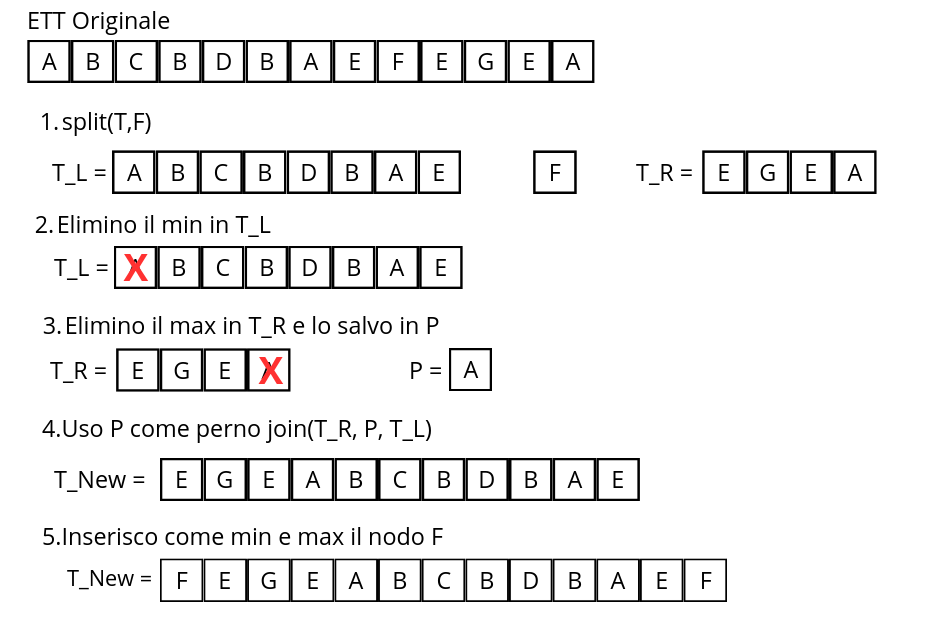
\includegraphics{rerootingEfficente.png}
    \caption[Titolo breve]{Procedura di rerooting}
    \labfig{rerootingEfficente}
\end{marginfigure}

\subsubsection{Link}

L'operazione di \textbf{link}$(u, v)$ permette di unire due alberi distinti attraverso l'introduzione di un nuovo arco $(u, v)$. Per garantire un'efficienza logaritmica, l'operazione viene implementata sfruttando le struttre dati precedentemente introdotte e l'operazione ausiliaria di \textit{rerooting}.

La procedura si articola nelle seguenti fasi:

\begin{enumerate}
    \item \textbf{Normalizzazione delle radici:} Si eseguono le operazioni $\text{rerooting}(T_1, u)$ e $\text{rerooting}(T_2, v)$ sui rispettivi Euler Tour Trees. Questa fase assicura che il tour di $T_1$ inizi nel nodo $u$ e quello di $T_2$ inizi nel nodo $v$, predisponendo le sequenze per la giunzione lineare.
    
    \item \textbf{Composizione della sequenza (Join):} Si crea un nuovo nodo dell'RB-Tree, denotato come $P = (u, v)$, che funge da arco di giunzione tra i due alberi. Si procede alla concatenazione delle sottosequenze tramite l'operazione di \textit{join}:
    \[ T_{new} = \text{join}(T_1, P, T_2) \]
    Il riferimento al nuovo arco $P$ viene contestualmente inserito nelle hash map $\textit{mapEdge}$ e solo se necessario in $\textit{mapNode}$ per consentire accessi futuri in tempo costante.

    \item \textbf{Chiusura del ciclo euleriano:} Per ristabilire la proprietà di ciclo della struttura risultante e mantenere $u$ come radice complessiva, è necessario introdurre un arco di ritorno. Si crea un nodo $P' = (v, u)$ e lo si inserisce come elemento massimo (ovvero in ultima posizione) della sequenza $T_{new}$, anche l'arco $P'$ viene registrato nella struttura di supporto $\textit{mapEdge}$.
\end{enumerate}

\begin{marginfigure}
    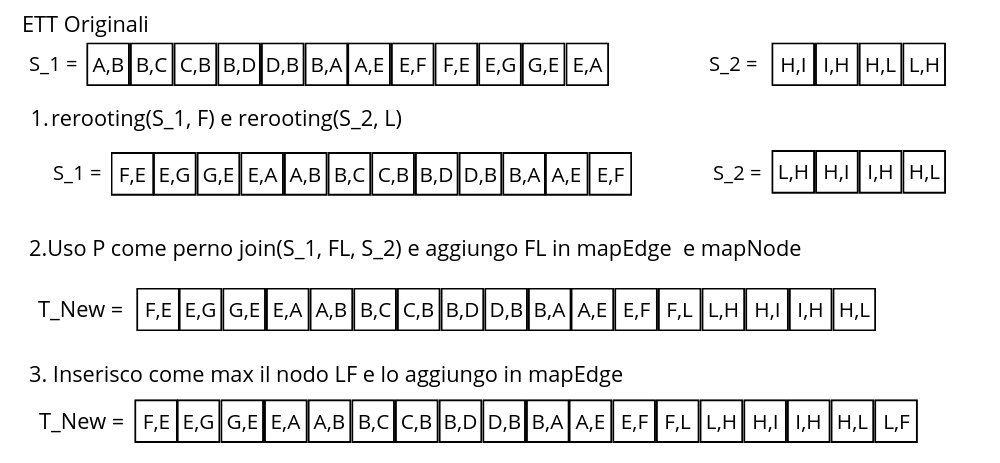
\includegraphics{linkEfficente.png}
    \caption[Titolo breve]{Procedura di link}
    \labfig{linkEfficente}
\end{marginfigure}

\subsubsection{Cut}
L'operazione di \textbf{cut}$(u, v)$ permette di separare un albero in due alberi distinti attraverso la cancellazione di un arco $(u, v)$. Per garantire un'efficienza logaritmica, l'operazione viene implementata sfruttando le struttre dati precedentemente introdotte e l'operazione ausiliaria di \textit{rerooting}.

La procedura si articola nelle seguenti fasi:

\begin{enumerate}
    \item \textbf{Primo accesso alla sequenza:}Si interroga la hash map $\textit{mapedge}[u,v]$ per ottenere il puntatore al nodo dell'RB-Tree che memorizza un arco $e_{del}=(u,v)$. Questa operazione garantisce la localizzazione del punto di taglio in tempo costante $O(1)$.
    \item \textbf{Prima decomposizione (Split):} Si esegue l'operazione di $\text{split}(T, e_{del})$ sulla sequenza originale. Tale operazione scinde l'albero $T$ in tre componenti distinte:
    \begin{itemize}
        \item $T_L$: sottosequenza contenente tutti gli archi che precedono $e_{del}$ nel tour corrente;
        \item $e_{del}$: il nodo stesso identificato come punto di rottura;
        \item $T_R$: sottosequenza contenente gli archi successivi a $e_{del}$.
    \end{itemize}
    \item \textbf{Secondo accesso alla sequenza:}Si interroga la hash map $\textit{mapedge}[v,u]$ per ottenere il puntatore al nodo dell'RB-Tree che memorizza un arco $e'_{del}=(v,u)$.
    \item \textbf{Seconda decomposizione (Split):}Si esegue l'operazione di $\text{split}(T_R, e'_{del})$. Tale operazione scinde l'albero $T_L$ in tre componenti distinte:
    \begin{itemize}
        \item $T'_L$: sottosequenza contenente tutti gli archi successivi a $e_{del}$ e precedenti a $'e_{del}$ nel tour originale;
        \item $e'_{del}$: il nodo stesso identificato come punto di rottura;
        \item $T'_R$: sottosequenza contenente gli archi successivi a $e'_{del}$.
    \end{itemize}
    \item \textbf{Rimozione del gancio:} Si estrae l'elemento situato all'estrema destra di $T'_R$, che denotiamo con $P$.

    \item \textbf{Ricomposizione della sequenza (Join):} Si procede alla ricomposizione della sequenza utilizzando $P$ come elemento di giunzione, si esegue:
    \[ T_{new} = \text{join}(T_L, P, T'_R) \]
\end{enumerate}
In questo modo abbiamo otternuo $T'_L$ che rappresenta il tour euleriana del sottoalbero radicato in $v$ e $T_{new}$ che rappresenta l'albero originale senza il sottoalbero $T'_L$

\begin{marginfigure}
    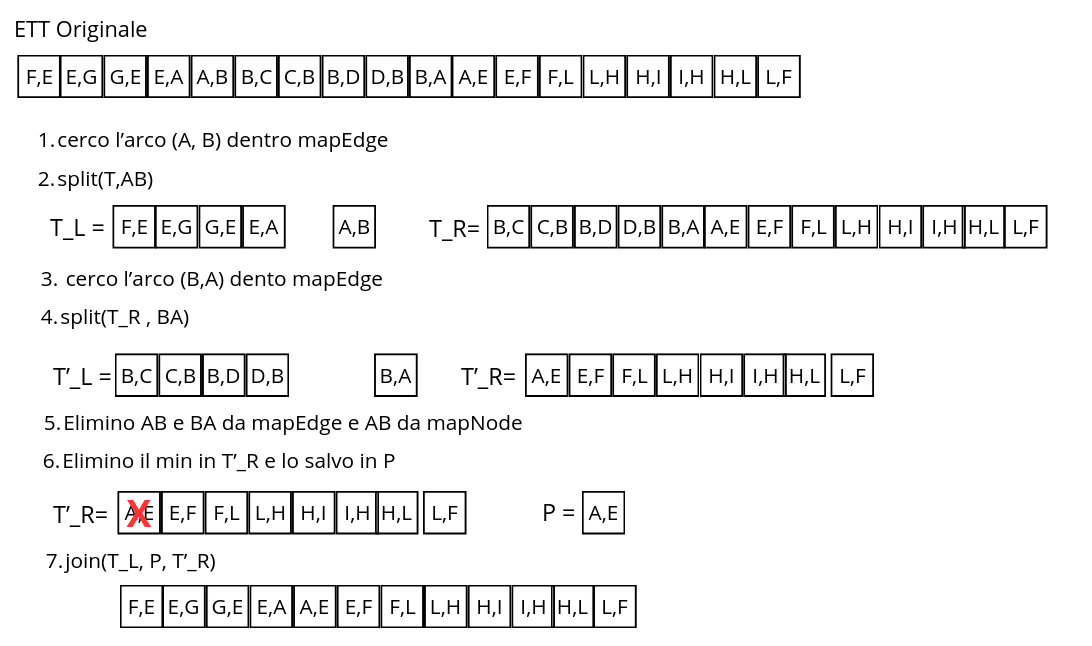
\includegraphics{cutEfficente.png}
    \caption[Titolo breve]{Procedura di cut}
    \labfig{cutEfficente}
\end{marginfigure}

%----------------------------------------------------------------------------------------

\backmatter % Denotes the end of the main document content
\setchapterstyle{plain} % Output plain chapters from this point onwards

%----------------------------------------------------------------------------------------
%   DEDICATION
%----------------------------------------------------------------------------------------
 
\thispagestyle{empty} 
\vspace*{\fill}
\begin{center}
    \itshape 
    The harmony of the world is made manifest in Form and Number, and the heart and soul and all the poetry of Natural Philosophy are embodied in the concept of mathematical beauty.\\
    \medskip
    --- D'Arcy Wentworth Thompson
\end{center}
\vspace*{\fill}
\clearpage

%----------------------------------------------------------------------------------------
%   BIBLIOGRAPHY
%----------------------------------------------------------------------------------------

% The bibliography needs to be compiled with biber using your LaTeX editor, or on the command line with 'biber main' from the template directory

\defbibnote{bibnote}{Here are the references in citation order.\par\bigskip} % Prepend this text to the bibliography
\printbibliography[heading=bibintoc, title=Bibliography, prenote=bibnote] % Add the bibliography heading to the ToC, set the title of the bibliography and output the bibliography note

%----------------------------------------------------------------------------------------
%   NOMENCLATURE
%----------------------------------------------------------------------------------------

% The nomenclature needs to be compiled on the command line with 'makeindex main.nlo -s nomencl.ist -o main.nls' from the template directory

\nomenclature{$c$}{Speed of light in a vacuum inertial frame}
\nomenclature{$h$}{Planck constant}

%----------------------------------------------------------------------------------------
%   GLOSSARY
%----------------------------------------------------------------------------------------

% The glossary needs to be compiled on the command line with 'makeglossaries main' from the template directory

\setglossarystyle{listgroup} % Set the style of the glossary (see https://en.wikibooks.org/wiki/LaTeX/Glossary for a reference)
\printglossary[title=Special Terms, toctitle=List of Terms] % Output the glossary, 'title' is the chapter heading for the glossary, toctitle is the table of contents heading

%----------------------------------------------------------------------------------------
%   INDEX
%----------------------------------------------------------------------------------------

% The index needs to be compiled on the command line with 'makeindex main' from the template directory

\printindex % Output the index

%----------------------------------------------------------------------------------------
%   BACK COVER
%----------------------------------------------------------------------------------------

% If you have a PDF/image file that you want to use as a back cover, uncomment the following lines

%\clearpage
%\thispagestyle{empty}
%\null%
%\clearpage
%\includepdf{cover-back.pdf}

%----------------------------------------------------------------------------------------

\end{document}